\chapter{RoFI Driver}\label{chap:software}

The RoFI platform does not give any restrictions on the implementation of
modules. However, having all the modules based on the same platform is an
advantage. Therefore, we consider the implementation of the universal module to
be a reference implementation of the other modules, and we expect the other
modules to reuse it as much as possibly.

Software development for robots and embedded systems is considered to be more
challenging than traditional software development. There are several reasons why
the development is challenging:
\begin{enumerate*}
    \item the microcontroller peripherals have to be mastered,
    \item testing and debugging is harder as the system is not self-contained
    and interacts with the environment, and
    \item the code has to deal with numerous asynchronous events, and there are
    tasks which need to be distributed in time.
\end{enumerate*}

We designed several tools and concepts to tackle these aspects of firmware
development and to make the development more convenient. We call them \emph{RoFI
Driver}. The driver is built on top of the software suite provided for the ESP32
microcontroller, which we sum up in section \ref{sec:hardware}. The driver
provides the following functionality:
\begin{itemize}
    \item it seamlessly integrates the docks into the software environment such
    that TCP/IP networking is available,
    \item the modules can distribute firmware updates automatically, and
    \item there is a low-level inter-module logging for debugging purposes.
    \item The driver also provides a high-level interface for controlling the
    motors and sensor. The interface allows for an easy handling of asynchronous
    events; and
    \item it is possible to do remote interface calls (i.e. to control another
    module).
\end{itemize}

\section{ESP32 Software Suite} \label{sec:hardware}

We expect the firmware for modules to be developed using standard programming
means for the ESP32 microcontroller. The firmware is developed using C++
facilitated by the ESP-IDF framework \cite{noauthor_esp-idf_nodate}. The
framework provides drivers for microcontroller peripherals. Therefore, the user
does not need to toggle individual bits in peripherals' registers. The framework
also includes FreeRTOS, the standard C and C++ libraries, and offers several
useful libraries (lwIP, Bluetooth library or library for a virtual file
system).

The framework exposes its functionality as a plain C interface. Also, many of
the provided functionality is wrapped in a POSIX-compatible interface. E.g.,
sockets are accessible by both, lwIP interface and POSIX interface. The same
follows for threading; the user can use FreeRTOS API or POSIX interface or can
even leverage C++ STL API.

\section{Networking} \label{sec:networking}

We leverage the lwIP library on the ESP32 to implement networking. This is
achieved by implementing a new network interface. All the docks in the module
appear as a single interface, therefore the interface performs simple switching
to determine the destination dock.

\subsection{Dock Integration}

Technically speaking, we have to provide following function to lwIP to implement
a new network interface:
\begin{itemize}
    \item \mintinline[breaklines]{c}{err_t rofi_if_init(struct netif *netif)}:
    to initialize the \texttt{nettif} structure,
    \item \mintinline[breaklines]{c}{err_t rofi_link_output(struct netif *netif, struct pbuf *p)}
    to transmit a complete datagram to the docks,
    \item \texttt{err\_t rofi\_if\_output(struct netif *netif, struct pbuf *p, ip\_addr\_t *ipaddr)}
    to wrap a datagram in custom headers and to transmit the datagram to the
    docks.
\end{itemize}
After system start, the RoFI driver calls \texttt{netif\_add}. The call register
a new network interface. After the setup, all the incoming datagrams are passed
to the \texttt{rofi\_netif->input} callback. The callback is set in the
structure by \texttt{netif\_add}. This is all, what is needed to integrate docks
to the lwIP library.

\subsection{Network Interface Implementation}

The implementation of the network interface is straightforward and rather
technical. There are only several aspects worth further comment:
\begin{enumerate*}
    \item mapping to content type and binary blobs of the dock interface defined
    in section \ref{sec:dock_interface},
    \item pairing destination address to docks, and
    \item the relation between switching and routing.
\end{enumerate*}

The docks can pass an arbitrary binary blobs to the mating side. The blobs are
marked by the content type specifier. The specifier allow us to transmit
multiple protocols through the same interface. In the RoFI driver, there are so
far 4 content type specifiers: 0 -- IP datagrams, 1 -- address mapping protocol
(defined further in this section), 2 -- low level logging (section
\ref{sec:logging}), and 3 -- firmware update protocol
(\ref{sec:firmware_distribution}).

In order to determine which dock should be used for a datagram transmission, a
mapping between destination IP addresses and outcoming dock is needed. The
mapping is performed by the ARP protocol \cite{plummer_ethernet_1982} in the
ethernet based networks. However, the ARP protocol is not a good choice in the
RoFI environment for the following reasons:
\begin{enumerate*}
    \item the connection between docks is point-to-point and
    \item the ARP protocol relies on MAC addresses of physical interfaces the
    docks do not provide.
\end{enumerate*}

Therefore, we design a simple \emph{address mapping protocol}. The protocol is
used to find IP addresses and GUIDs of the module neighbors. There are two
messages in the protocol: \emph{mapping call} and \emph{mapping response}. The
mapping call follows the format:

\bigskip
\begin{bytefield}[bitwidth=1.75em]{16}
    \bitheader{0,7} \\
    \bitbox{8}{command (0)}
\end{bytefield}

\noindent The response follows the format:

\bigskip
\begin{bytefield}[bitwidth=1.75em]{16}
    \bitheader{0,7,8,15} \\
    \bitbox{8}{command (1)} & \bitbox{8}{IP address size} \\
    \bitbox{8}{GUID size} & \bitbox{8}{number of entries ($n$)} \\
    \wordbox{2}{IP address 1} \\
    \wordbox{2}{module GUID 1} \\
    \wordbox{2}{$\vdots$} \\
    \wordbox{2}{IP address $n$} \\
    \wordbox{2}{module GUID $n$} \\
\end{bytefield}

Each module keeps a table for each dock with IP addresses and module GUIDs. Even
there is point-to-point communication, we allow for several entries. There are
following reasons to do that that: it allows to cluster modules in a system and
perform packet switching in the cluster if the further development finds it
suitable (e.g., packet switching has lower latency), and there can be simple
modules in the system not capable of routing (e.g., battery module). The
overhead caused by extended packet format is negligible and is worth further
extensibility.

On dock connection, the module actively sends the mapping response message to
the mating side. If there is a change making the information sent previously
invalid, a new message is sent (e.g. the module has changed its IP address). The
event driven approach allows to establish the mapping quickly. To avoid the
table to contain out-of-date information, the module should periodically use the
mapping call to update it. Note that under normal conditions the table cannot go
out-of-date; it can happen only when malfunction occurs (e.g., module resets).

\subsection{Module Address Configuration and Routing}

To communicate in the IP network, each module has to have a unique and valid IP
address. The modules have their own unique GUIDs, however, GUID is not a good
candidate for an IP address. First, it is longer than IPv4 address, second, it
does not follow standard format of IPv6 address, which reflects the structure of
the network, and therefore, GUID does not allow for efficient routing. There is
no central authority in the network of RoFIs, like there is a router in
traditional network. Traditional solutions for network address obtaining, like
DHCP server, cannot be used. Both, address configuration and routing in large
networks with unstable topology are still an area of active research and there
is no wide spread solution (\cite{baccelli_ip_2010} and
\cite{ezzouhairi_ip_2005}).

As the RoFI is built on top the TCP/IP networking, nearly all newly proposed
algorithms for routing (e.g., APM \cite{ezzouhairi_ip_2005}) can be adopted as
their experimental implementation relies on TCP/IP. The same goes for IP address
configuration, e.g, in form od Distributed DHCP server
\cite{nesargi_manetconf:_2002}. However, in the first versions of RoFI driver,
we rely on the basic address auto configuration and basic routing implemented in
lwIP. These algorithms work fine in small networks. In the future, we plan to
adopt the Distributed DHCP server and the APM routing algorithm.

\section{Low Level Logging} \label{sec:logging}

When a firmware for a microcontroller is developed, programmers usually use a
simple communication interface, typically UART, to print debugging messages.
This is useful, as most systems cannot be paused by a debugger as it is
impossible to pause surrounding environment. UART is usually used as it is
stateless, has nearly no code dependencies and is easy to setup.

The same approach can be used for a debugging of a single unit, however
collecting data from multiple UART on multiple modules is rather impractical.
TCP/IP sockets can be used, however, in case of routing malfunction or system
crash a message cannot be delivered. Therefore, we introduce \emph{low level
logging} in the RoFI driver -- a simple and robust protocol for sending messages
in a RoFI system.

The low level logging is implemented directly on top of the dock interface and
does not rely on TCP/IP networking. The goal is to emmit a string and propagate
it to all modules or a special debugging adapter in a form of dock, where it can
be transmitted to the programmer. The protocol should be used only for debugging
purposes and should be disabled in release builds as it is build on a naive
flooding algorithm.

The low level debugging uses content type specifier 2 (section
\ref{sec:dock_interface}). There is only one type of message:

\bigskip
\begin{bytefield}[bitwidth=1.75em]{16}
    \bitheader{0,15} \\
    \wordbox{2}{message string}
\end{bytefield}

\noindent The string can have length up to 65535 bytes. There is a set of string
hashes in each modules. The set keeps hashes of all received messages. When a
module receives a string it calculates its hash. If the hash is not present in
the set, it is inserted and the string is resend to all other docks in the
module. The hashes in the set expire after a given period of time. Expired
hashes are removed from the set. This algorithm ensures all emitted messages are
spread into the whole system. Note, that if the expiration period is too short,
is is possible to create a message going through the system indefinitely.
However, for the debugging purposes we do not perceive it as a limitation.

\section{Automatic Firmware Distribution} \label{sec:firmware_distribution}

It is highly desirable that all modules of the same type run the same firmware
version. If the modules are able to synchronize firmware automatically, the
development process can be speed up. The firmware distribution can be achieved
in two ways -- either there is central authority publishing the firmware, or the
modules check firmware of their neighbors and update the firmware from them.

ESP32 is a suitable microcontroller for remote firmware upgrades. Traditional
microcontrollers can update their firmware only using bootloader, a small
program in reserved are of flash memory executed after microcontroller boot. If
there is need for custom update protocol, custom bootloader should be written.
However, bootloaders have to be self-contained and have restricted binary size,
therefore sophisticated update protocols are hard implement. This is not the
case for ESP32 \cite{noauthor_esp-idf_nodate}. The flash memory of ESP32 can be
divided in partitions (e.g., firmware or virtual file system partition). In the
default configuration, there are two partition for firmware. These partitions
are used to implement \emph{over-the-air updates} (OTA). One partition is marked
as an active an and upon boot, the bootloader loads user firmware from the
active partition. Then, during a regular operation of the microcontroller,
firmware can be written in the second, inactive, partition. Once the firmware is
written and validated, the active flag of the partitions is swapped. When the
microcontroller reboots, new firmware is used. OTA updates allow to use existing
codebase in the firmware to perform firmware updates. Therefore complicated
protocols, like update from an HTTP server can be implemented.

ESP-IDF provides implementation of OTA update from HTTP server and interface for
implementing custom updates. The update from HTTP server works by specifying URL
and periodical polling for new firmware version. The interface consists of three
functions -- one for starting the update, one for processing a binary blob with
a piece of firmware, and one for committing the changes.

The HTTP server update is an example of a central update. We find it unsuitable
for the RoFI systems for following reasons:
\begin{enumerate*}
    \item each module downloads the firmware separaMožná jo, tely and therefore the
    protocol does not scale well, and
    \item it relies on working TCP/IP connection and routing. If a firmware
    update breaks routing, the firmware update stops working.
\end{enumerate*}
Therefore, we introduce a decentralized \emph{firmware update protocol} relying
only on dock connection. By flashing a single module, its firmware distributes
among the other modules in a system. We do not restrict the flashing procedure
-- it can be either flashed by a cable from a PC or the module can download its
firmware from a central authority (therefore, a hybrid approach can be
achieved).

The protocol works as follows. Each firmware has built in two symbols in the
binary: \texttt{ROFI\_FW\_TYPE} and \texttt{ROFI\_FW\_TIMESTAMP}. Firmware type
is specified by the user, timestamp is automatically added during build.
Firmware type is a 16-bit unsigned integer, timestamp is a 64-bit unsigned
integer. There are no restrictions on meaning of the numbers; it is recommended
that the timestamp are milliseconds since UNIX time epoch. A module updates only
to the same firmware type as it already is and to a newer timestamp. The
firmware type allow the system can consist of various type of modules.

The firmware update protocol uses content type specifier 3 (section
\ref{sec:dock_interface}). There are four type of messages:

\paragraph{Firmware request} is sent by a module to find out firmware version of
its neighbors. The answer is firmware announcement. The message has the
following format:

\bigskip
\begin{bytefield}{32}
    \bitheader{0, 7} \\
    \bitbox{8}{command (0)}
\end{bytefield}

\paragraph{Firmware announcement} is broadcasted by a module to its direct
neighbors, when it knows new firmware. The firmware might not be completely
known to the module and therefore, there is a field known size in the message.
If more of the firmware code is known, new message is broadcasted. The message
has the following format:

\bigskip
\begin{bytefield}{32}
    \bitheader{0, 7, 8, 15, 16, 31} \\
    \bitbox{8}{command (1)} & \bitbox{8}{\textit{reserved}} & \bitbox{16}{firmware type} \\
    \wordbox{2}{firmware timestamp} \\
    \bitbox{32}{firmware size} \\
    \bitbox{32}{known size}
\end{bytefield}

\paragraph{Firmware chunk request} is sent by a module to obtain a new chunk of
the firmware. It is usually a response to firmware announcement. The chunks are
1024 bytes in length (except the last one) and the allowed offsets are also in
multiplies of 1024. The message has the following format:

\bigskip
\begin{bytefield}{32}
    \bitheader{0, 7, 8, 15, 16, 31} \\
    \bitbox{8}{command (2)} & \bitbox{8}{\textit{reserved}} & \bitbox{16}{firmware type} \\
    \wordbox{2}{firmware timestamp} \\
    \bitbox{32}{chunk offset}
\end{bytefield}

\paragraph{Firmware chunk response} is a response to firmware chunk request. The
message has the following format:

\bigskip
\begin{bytefield}{32}
    \bitheader{0, 7, 8, 15, 16, 31} \\
    \bitbox{8}{command (3)} & \bitbox{8}{\textit{reserved}} & \bitbox{16}{firmware type} \\
    \wordbox{2}{firmware timestamp} \\
    \bitbox{32}{chunk offset} \\
    \bitbox{32}{chunk length} \\
    \wordbox{2}{chunk data}
\end{bytefield}

\noindent First, we illustrate the protocol operation in a system composed of
single module type. Then, we extend it to an arbitrary RoFI systems.

When a first module receives a new firmware, it broadcast the firmware
announcement. Each module keeps a record of the source of newest firmware
available. It can be either the module itself, or one of its neighbors. The
firmware sources are ordered by timestamp and known size and for now, we ignore
firmware types. If a module receives firmware announcement, it checks if it is
newer. If not, the message is ignored. Otherwise it updates the firmware source.
When a firmware source contains newer firmware than the firmware the module
currently runs, it starts the upgrade procedure. It uses firmware chunk request
to ask the firmware source for a new firmware chunk. If newer source of firmware
appears, the current firmware update is aborted and new update is started.
During the update, the module itself broadcasts firmware announcement message as
new chunks of firmware are received. In this fashion, the new firmware spreads
like a wave in the system. Note, that messages can loose in the system as docks
are allowed to drop datagrams. Therefore, if message response times out, the
module broadcasts firmware request to find a new firmware source.

To support multiple firmware types, the module keeps track of newest firmware
available for each type. If firmware announcement updates other type of firmware
than module type, it broadcasts the announcement to all neighbors. If firmware
chunk request for other firmware is received, it is redirected to the the source
of that type of firmware and remembers the request. When a response in form of
firmware chunk is received, the module redirects the message to the author of
the request.

\section{Reactive Blocks Library} \label{sec:rbl}

There are currently two classical approaches to tackle the burden of handling
asynchronous events in languages like C or C++. First, a real-time operating
system (RTOS) can be used with several tasks. Each task handles events in
synchronous, blocking, manner. This approach leads to a readable code as the
logic for processing events is kept close together and follows the chronological
flow of the events. However, it might not preserve the lowest possible latency
due to RTOS task switching and also does not scale well as each the number of
tasks is usually limited. The second approach uses callback functions which are
called to handle an event. This approach scales well; however it leads to a
hard-to-read code as the callbacks do not preserve context and are spread all
over the source code. This phenomenon is usually referred to as ``callback
hell''. Also, code complexity increases tremendously when error handling is
added.

We designed a new solution for handling asynchronous events for the RoFI
platform. We call it \emph{reactive blocks}. The idea behind reactive blocks is
simple -- we use the same principle as callbacks; however, we provide a
syntactical sugar to write them in a chain-like structure to preserve the
chronological flow of event handling. Reactive blocks are inspired by the
ReactiveX library \cite{noauthor_reactivex_nodate} and the ranges-v3 library
\cite{noauthor_range-v3_nodate}.

The reactive blocks will be implemented as a stand-alone RoFi independent C++
library -- \emph{Reactive Blocks Library} (RBL). The library targets all
platforms with C++17 and STL support. The target platforms include standard
variants of x64, ARM and also embedded platforms like ESP32 or ARM Cortex-M. As
the library implementation is a subject of another thesis, we provide only a
brief description of its core functionality and omit some semantical nuances and
the implementation details.

Consider following (somewhat artificial) scenario: when a noisy distance sensor
overcomes a given threshold (generates edge), the robot notifies several other
robots (judges) over a network. The judges vote and if a majority votes yes, the
robot flashes a LED. For simplicity, consider a line-based text communication
protocol between the robots and numerous reasonably named functions.

Standard implementation using blocking interface might look like this:
\begin{minted}{cpp}
while ( true ) {
    // Wait rising edge debounced by 10 samples
    ring_buffer< int > samples( 10, 0 );
    while ( !all( samples,
                  []( int x ){ return x > threshold; } ) )
    {
        samples.push( sensor.read() );
        delay( 10_ms );
    }
    int sensorValue = average( samples );

    // Perform voting
    std::vector< bool > votes;
    for ( auto& judge : judges ) {
        judge.send( "value: " + std::to_string( sensorValue ) )
        vote = judge.receiveLine() == "yes";
        votes.push_back( vote );
    }

    // Flash an LED
    if ( majority( votes, []( bool vote ){ return vote; } ) ) {
        led.on();
        delay( 200_ms );
        led.off();
    }
}
\end{minted}

The sample code is straightforward and easily readable. By putting the code in a
separate task, we can handle multiple asynchronous events simultaneously.
However, the code does is not as efficient as possible as the network
communication is synchronous.

Each asynchronous function traditionally takes a callback function as its
argument. The callback is called, when the operation is finished. The result
value or error is passed to the callback. The task from our example scenario
could be implemented like this using asynchronous interface:

\begin{minted}{cpp}
std::vector< bool > votes;
template < typename Callback >
void onJudgeResponse( const std::string& resp, Callback c ) {
    votes.push_back( resp == "yes" );
    if ( votes.size() == judges.size() &&
         majority( votes, []( bool vote ){ return vote; } ) )
    {
        c();
    }
}

template < typename Callback >
void vote( int value, Callback c ) {
    for ( auto& judge : judges ) {
        judge.send( "value: " + std::to_string( sensorValue ), [=] {
            judge.receiveLine( [=]( const std::string& s ) {
                onJudgeResponse( resp, s, c );
            } );
        } );
    }
}

ring_buffer< int > samples( 10, 0 );
timer.every( 10_ms. [&ring_buffer]() {
    samples.push( sensor.read() );
    if ( all( samples,
        []( int x ){ return x > threshold; } ) )
    {
        vote( average( samples ), judges, []{
            led.on();
            timer.after( 200_ms, []{
                led.off();
            });
        });
    }
});
\end{minted}

The code is now fully asynchronous, but is hard to read -- it does not preserve
the chronological order of event handling, the user have to think about shared
states and has a lot of nested sections. The need for a shared state arises from
the absence of information in the control flow of the program. E.g, the function
\texttt{onJudgeResponse} has to check if it is the last call of the function. In
the first example there is no such need as the the control captures the
information -- once the if-clause is reached, it is clear all judges voted.

The solution we provide is shown in code snippet below. We do not expect the
reader to immediately understand all details of the code as explanation
follows. We advise the reader to return to this example during the rest of
this section.

\begin{minted}{cpp}
auto overThreshold( std::pair< int, int > value ) {
    return value.first > threshold;
}

auto is( const std::string& what ) {
    return [=]( const std::string& s ) { return s == what; }
}

auto setLed( bool value ) {
    return [=]() { led.set( value ) };
}

auto sensorStream = timer.every( 20_ms ) >> sensor.read;
auto sensorAverage = sensorStream >> slidingAverage( 10 );
zip( sensorStream, sensorAverage)
    >> debounceOn( overThreshold )
    >> std::get< 1 >
    >> [&]( int sensorValue ) {
        return interleave( judges, [=]( auto& judge ) {
            std::string msg =
                "value: " + std::to_string( sensorValue );
            return judge.send( message )
                    >> judge.receiveLine >> is( "yes" );
        } ) >> majority;
    }
    >> setLed( true ) >> wait( 200_ms ) >> setLed( false );
\end{minted}

The reactive blocks follow similar idea as the range-v3 library -- we describe a
pipeline for data transformation, however unlike ranges-v3, the data might be
scattered over time. By describing the pipeline the user can preserve
chronological ordering of the event handling in the code but also preserves
asynchronicity at the same time. In the traditional future concept, which also
allows to describe a pipeline, the pipeline is only linear and allows only a
single value to pass. The reactive blocks allow for non-linear pipelines and
also allows multiple values to pass through it. Visualization of the pipeline
for the example above is shown in figure \ref{fig:rbl_example_1}.

\begin{figure}[!t]
    \centering
    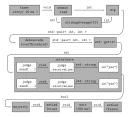
\includegraphics[]{figures/rbl_pipeline_1.pdf}
    \caption{Pipeline visualization for sensor and voting code snippet.}
    \label{fig:rbl_example_1}
\end{figure}

Reactive blocks allow chaining data transformation operations -- just like UNIX
pipe operator. A block represents each operation. There are two type of blocks:
\mintinline[breaklines]{cpp}{template < typename T > Puslisher< T > } and
\mintinline[breaklines]{cpp}{template < typename T > Subscriber< T > }. Single
block can be both publisher and subscriber.

\noindent The publisher can:
\begin{enumerate}
    \item emit an arbitrary number of values of type \texttt{T} at any time (we
    say it generates a \emph{stream} of values),
    \item emit an error (object inheriting from
    \mintinline[breaklines]{cpp}{std::exception}), and
    \item close itself (mark the end of its stream). After closing no more
    values nor errors can be emitted.
\end{enumerate}

\noindent The subscriber can subscribe to a publisher. After subscribing it
\begin{enumerate}
    \item receives values of type \texttt{T} emitted by the publisher and
    \item can unsubscribe.
\end{enumerate}

The interface of subscriber and publisher is provided in the
following snipped:
\begin{minted}{cpp}
template < typename T >
class Publisher {
public:
    void subscribe( Subscriber< T >* s );
    void unsubscribe( Subscriber< T >* s );
protected:
    void publish( T t );
    void publishError( const std::exception& e );
    void close();
};

template < typename T >
class Subscriber {
protected:
    virtual void onValue( T t ) = 0;
    virtual void onError( const std::exception& e ) = 0;
    virtual void onClose() = 0;
};
\end{minted}

With these base classes we can derive any other reactive block. For example we
can build a block which converts a number to a string:
\begin{minted}{cpp}
class N2S: public Publisher< std::string >,
    public Subscriber< int >
{
    virtual void onValue( int i ) override {
        publish( std::to_string( i ) );
    }
    virtual void onError( const std::exception& e ) override {
        publishError( e );
    }
    virtual void onClose() override {
        close();
    }
};
\end{minted}

Or, given a classical callback-based asynchronous interface in form of function
\mintinline[breaklines]{cpp}{errorCode asyncFoo( int param, Callback c )} we can
wrap it inside a block which accepts the input for the asynchronous function and
produces an output.
\begin{minted}{cpp}
class AsyncFoo: public Publisher< int >,
    public Subscriber< int >
{
    virtual void onValue( int i ) override {
        errorCode = asyncFoo( i, [&]( int retval ) {
            this->publish( retval );
        } );
        if ( errorCode == ERROR )
            publishError(
                std::runtime_exception( "Something wrong" ) );
    }
    virtual void onError( const std::exception& e ) override {
        publishError( e );
    }
    virtual void onClose() override {
        close();
    }
};
\end{minted}

In similar manner, all asynchronous events can be wrapped inside a reactive
block -- including interrupts or possibly, but not preferably, busy waiting.
Note, that the reactive blocks does not bring asynchonicity in the system, they
just provide a new interface for it. The blocks can also wrap synchronous tasks
as shown in the example of the \texttt{N2S} class. The only requirement is that
the code inside a block should not block for a long time as it might delay other
pending blocks. Also, there can be $m$-to-$n$ mapping of incoming values to the
block, not just 1:1 mapping as we showed in the examples. The block can emit
multiple values from a single input value (e.g., block splitting string
according to a delimiter or timer producing values at a given period).

When multiple blocks are linked together via the subscribe relation, we call the
final structure chain. Therefore, we will refer to the operation as
\emph{chaining blocks}. Chains are first-class citizens just like blocks.
Therefore we can store them in variable or chain multiple chains together.

However, building the block manually by defining classes is verbose and leads to
hard-to-read code. Therefore, the library provides operator
\mintinline[breaklines]{cpp}{>>} (chain). The operator is similar to Haskell's
bind operator -- it builds the subscribe relation between chains. The operator
comes in many overloads and provides implicit creation of blocks out of
functions. This functionality provides a syntactical sugar, which allows to make
the code less verbose and also allows to keep the code in chronological order.

To further simplify the code, the library should provide predefined blocks like
zip (takes two streams of values and combines them together in pairs),
interleave which takes multiple streams and joins them together, simple waiting,
and so forth.

The last advantage of reactive blocks we present is error handling. The
publishers can publish value or an error. By default, the error goes through the
pipeline until some block stops it and handles it. This provides a monadic- and
exception-like behavior. See following example:
\begin{minted}{cpp}
a >> b >> c >> onError( []( std::exception& e ) {
    std::cerr "Error a-c: " << e.what() << std::endl();
} ) >> d >> e >> onError( []( std::exception& e ) {
    std::cerr "Error d-e: " << e.what() << std::endl();
} );
\end{minted}
The code defines a linear chain of blocks \texttt{a} to \texttt{e}. If any of
the block fails, the error is captured by one the two error handlers. Also, the
chain operator by default captures exception thrown out of functions and sends
them down the chain:
\begin{minted}{cpp}
a >> [] {
    throw std::runtime_error( "Inevidable error" );
} >> b >> onError( []( std::exception& e ) {
    std::cerr "Inevidable error follows:  "
        << e.what() << std::endl();
} );
\end{minted}

In the text above, we presented the library using a runtime polymorphism, which
might not be suitable for embedded platforms. However, for chains with a type
known in the compile time the runtime polymorphism could be eliminated in the
future releases of the library. The runtime polymorphism elimination also allow
for further optimization and reducing the cost of the reactive blocks
abstraction.

\section{RoFI Driver Interface}
